% ============================================================================
%  MEMORIA ACADÉMICA — DOOM AUV Simulation
%  Compilar con: pdflatex Memoria_DOOM_AUV.tex  (x2 para referencias)
%  Requiere: texlive-publishers (para IEEEtran) o usar article como fallback
% ============================================================================
\documentclass[10pt,twocolumn,letterpaper]{article}

% ----- Paquetes -----
\usepackage[utf8]{inputenc}
\usepackage[T1]{fontenc}
\usepackage[spanish]{babel}
\usepackage{times}
\usepackage{graphicx}
\usepackage{amsmath,amssymb}
\usepackage{hyperref}
\usepackage{url}
\usepackage{booktabs}
\usepackage{multirow}
\usepackage{xcolor}
\usepackage{listings}
\usepackage{float}
\usepackage{caption}
\usepackage{subcaption}
\usepackage{geometry}
\usepackage{titlesec}
\usepackage{enumitem}
\usepackage{fancyhdr}
\usepackage{abstract}

\geometry{letterpaper, left=1.8cm, right=1.8cm, top=2.2cm, bottom=2.2cm}

% ----- Configuración de listings -----
\definecolor{codebg}{rgb}{0.95,0.95,0.97}
\definecolor{codegreen}{rgb}{0.0,0.5,0.0}
\definecolor{codegray}{rgb}{0.5,0.5,0.5}
\definecolor{codepurple}{rgb}{0.58,0,0.82}

\lstdefinestyle{pythonstyle}{
    backgroundcolor=\color{codebg},
    commentstyle=\color{codegreen},
    keywordstyle=\color{blue}\bfseries,
    numberstyle=\tiny\color{codegray},
    stringstyle=\color{codepurple},
    basicstyle=\ttfamily\scriptsize,
    breakatwhitespace=false,
    breaklines=true,
    captionpos=b,
    keepspaces=true,
    numbers=left,
    numbersep=4pt,
    showspaces=false,
    showstringspaces=false,
    showtabs=false,
    tabsize=2,
    frame=single,
    rulecolor=\color{codegray},
    language=Python
}
\lstset{style=pythonstyle,
  literate=
    {á}{{\'{a}}}1 {é}{{\'{e}}}1 {í}{{\'{i}}}1 {ó}{{\'{o}}}1 {ú}{{\'{u}}}1
    {Á}{{\'{A}}}1 {É}{{\'{E}}}1 {Í}{{\'{I}}}1 {Ó}{{\'{O}}}1 {Ú}{{\'{U}}}1
    {ñ}{{\~{n}}}1 {Ñ}{{\~{N}}}1
}

% ----- Formato de secciones -----
\titleformat{\section}{\large\bfseries}{\thesection.}{0.5em}{}
\titleformat{\subsection}{\normalsize\bfseries}{\thesubsection}{0.5em}{}
\titleformat{\subsubsection}{\small\bfseries\itshape}{\thesubsubsection}{0.5em}{}

% ----- Metadatos -----
\hypersetup{
    colorlinks=true,
    linkcolor=blue!70!black,
    citecolor=blue!70!black,
    urlcolor=blue!70!black,
    pdftitle={Simulación de AUV con Arquitectura ROS2 y Motor de Renderizado DOOM},
    pdfauthor={Sergio}
}

% ============================================================================
\begin{document}

% ----- Título -----
\twocolumn[
\begin{@twocolumnfalse}
\begin{center}
    {\LARGE\bfseries Simulación de un Vehículo Autónomo Submarino \\
    con Arquitectura Distribuida ROS\,2 y Motor de \\
    Renderizado en Primera Persona Estilo \textit{DOOM}\par}
    \vspace{0.8em}
    {\large Sergio --- al428707@uji.es\par}
    \vspace{0.3em}
    {\normalsize Universitat Jaume I --- Grado en Ingeniería\\
    Asignatura: Aéreos y Submarinos\par}
    \vspace{0.3em}
    {\normalsize Febrero 2026\par}
    \vspace{1.2em}
\end{center}

% ----- Abstract -----
\begin{onecolabstract}
\noindent
El presente trabajo describe el diseño, implementación y validación de \textbf{DOOM AUV Sim}, un simulador completo de Vehículo Autónomo Submarino (AUV) construido sobre el \textit{middleware} ROS\,2 Humble y el lenguaje Python. El sistema integra un motor de renderizado en primera persona basado en \textit{raycasting} 2.5D ---inspirado en el videojuego \textit{DOOM} (1993)---, un motor de física subacuática con inercia hidrodinámica y consumo de batería, un canal de comunicación acústica submarina con latencia y pérdida de paquetes modeladas según la fórmula de absorción de Thorp, y un módulo de autonomía \textit{onboard} con arquitectura de control inspirada en la subsunción de Brooks. La arquitectura distribuida emplea seis nodos ROS\,2 interconectados mediante aproximadamente veinte tópicos \textit{Pub/Sub}, sin recurrir a Servicios ni Acciones, lo cual se justifica por la naturaleza asíncrona y con latencia variable del dominio submarino. El sistema fue desarrollado de manera iterativa a lo largo de múltiples ciclos de diseño-implementación-prueba, resolviendo progresivamente problemas de estabilidad del control de profundidad, alineación del brazo robótico, comunicación acústica realista y captura de objetivos. Los resultados demuestran que el simulador permite la recolección autónoma de cinco objetivos distribuidos aleatoriamente, la evasión reactiva de obstáculos dinámicos y estáticos, y la exportación del mapa explorado en formatos PCD, PNG y OBJ.
\end{onecolabstract}
\vspace{1em}
\end{@twocolumnfalse}
]

% ============================================================================
\section{Introducción}
\label{sec:introduccion}

Los Vehículos Autónomos Submarinos (AUV, \textit{Autonomous Underwater Vehicles}) representan una de las plataformas robóticas más desafiantes en ingeniería. A diferencia de los robots terrestres o aéreos, los AUV operan en un entorno donde la comunicación electromagnética convencional ---incluido el GPS--- resulta inviable más allá de unos pocos metros de profundidad. La alternativa estándar, la comunicación acústica submarina, introduce latencias del orden de cientos de milisegundos a segundos y tasas de pérdida de paquetes significativas, limitando severamente la capacidad de teleoperación en tiempo real~\cite{stojanovic2009}.

En este contexto, el desarrollo de simuladores que reproduzcan fielmente estas restricciones operativas constituye una necesidad crítica tanto para la formación de operadores como para la validación de algoritmos de autonomía. Sin embargo, la mayoría de simuladores de AUV existentes ---tales como UUV Simulator~\cite{uuvsim2016} o Stonefish~\cite{stonefish2020}--- se centran en la fidelidad física del medio subacuático o en la integración con marcos de planificación como Nav2, pero no necesariamente exponen al usuario las limitaciones perceptuales y comunicacionales del robot de manera intuitiva.

El presente proyecto propone un enfoque alternativo: un simulador de AUV que utiliza un motor de renderizado en primera persona inspirado en el clásico DOOM (id Software, 1993) para representar de forma inmersiva la perspectiva limitada del sonar frontal del vehículo. Este \textit{raycasting} 2.5D, combinado con un sistema de \textit{fog of war} (niebla de guerra), obliga al operador a experimentar las mismas restricciones sensoriales que el AUV real, facilitando la comprensión intuitiva de sus capacidades y limitaciones.

El sistema fue construido íntegramente sobre ROS\,2 Humble, aprovechando su modelo de comunicación \textit{Pub/Sub} para implementar una arquitectura distribuida de seis nodos que separa claramente las responsabilidades de simulación, comunicación, arbitraje, autonomía y visualización. A lo largo de su desarrollo iterativo, se abordaron y resolvieron múltiples desafíos técnicos relacionados con la estabilidad del control, la fidelidad del canal acústico y la coordinación del brazo robótico.

% ============================================================================
\section{Estado del Arte}
\label{sec:estado_arte}

\subsection{Simulación de AUV en ROS\,2}

El ecosistema ROS\,2 ofrece diversas opciones para la simulación de vehículos submarinos. El paquete UUV Simulator~\cite{uuvsim2016}, originalmente desarrollado para ROS\,1, proporciona modelos hidrodinámicos detallados en Gazebo, pero su complejidad de configuración y los requisitos computacionales de la simulación física tridimensional completa lo hacen poco adecuado para iteración rápida. Stonefish~\cite{stonefish2020} ofrece un simulador más ligero con soporte nativo para ROS\,2, pero sigue requiriendo modelos URDF, archivos de mundo y configuración de sensores complejos.

Estos simuladores priorizan la fidelidad física por encima de la accesibilidad y la rapidez de prototipado. En contraste, el enfoque adoptado en este trabajo privilegia la \textbf{fidelidad funcional}: se replican los efectos operativos (latencia, pérdida de paquetes, campo de visión limitado, inercia) sin necesidad de una simulación física tridimensional completa.

\subsection{Comunicación Acústica Submarina}

La propagación del sonido bajo el agua está gobernada por fenómenos de absorción dependiente de la frecuencia, dispersión geométrica y efectos de canal variable. La fórmula de Thorp~\cite{thorp1967} proporciona una aproximación práctica al coeficiente de absorción $\alpha$ en dB/km para una frecuencia $f$ en kHz:

\begin{equation}
\alpha = \frac{0.11 f^2}{1 + f^2} + \frac{44 f^2}{4100 + f^2} + 2.75 \times 10^{-4} f^2 + 0.003
\label{eq:thorp}
\end{equation}

La pérdida por transmisión (\textit{Transmission Loss}, TL) combina la dispersión geométrica y la absorción:

\begin{equation}
TL = 20 \log_{10}(R) + \alpha \cdot R \cdot 10^{-3} \quad [\text{dB}]
\label{eq:tl}
\end{equation}

donde $R$ es la distancia en metros. La relación señal-ruido (SNR) resultante se calcula como $\text{SNR} = SL - TL - NL$, siendo $SL$ el nivel de fuente y $NL$ el nivel de ruido ambiental~\cite{urick1983}.

\subsection{Arquitectura de Subsunción}

La arquitectura de subsunción, propuesta por Brooks~\cite{brooks1986}, organiza el control robótico en capas de comportamiento con prioridad estricta. Las capas inferiores (comportamientos reactivos de supervivencia) pueden \textit{suprimir} las salidas de capas superiores (comportamientos orientados a objetivos). Este paradigma resulta especialmente apropiado para entornos dinámicos e impredecibles como el fondo marino, donde la evasión de obstáculos debe tener prioridad absoluta sobre cualquier objetivo de misión.

% ============================================================================
\section{Hipótesis y Diseño}
\label{sec:hipotesis}

La hipótesis central de este trabajo es que un \textbf{simulador de AUV ligero, basado exclusivamente en comunicación Pub/Sub de ROS\,2 y con renderizado 2.5D}, puede reproducir las restricciones operativas esenciales de un vehículo submarino real ---latencia acústica, percepción limitada, inercia hidrodinámica--- con la fidelidad funcional suficiente para validar algoritmos de autonomía y entrenar operadores, sin requerir la complejidad de un simulador físico tridimensional completo.

El diseño se fundamenta en tres premisas:

\begin{enumerate}[leftmargin=*,itemsep=2pt]
    \item \textbf{Separación estricta simulación-control:} El motor de simulación publica \textit{ground truth} en tópicos aislados (\texttt{/sim/*}), y un nodo puente introduce delay antes de republicarlos como percepción del AUV (\texttt{/auv/*}).
    \item \textbf{Comunicación realista como requisito, no como opción:} Todos los comandos del operador deben atravesar el canal acústico simulado. No existen atajos de comunicación directa.
    \item \textbf{Seguridad por subsunción:} Los comportamientos de evasión de obstáculos y \textit{failsafe} de batería pueden anular tanto la autonomía como el control manual.
\end{enumerate}

% ============================================================================
\section{Metodología}
\label{sec:metodologia}

\subsection{Arquitectura General del Sistema}

El sistema se compone de seis nodos ROS\,2 propios, un nodo de visualización externo (RViz\,2) y un nodo de teleoperación ejecutado en terminal independiente. La Figura~\ref{fig:topologia} presenta la topología completa.

\begin{figure}[H]
    \centering
    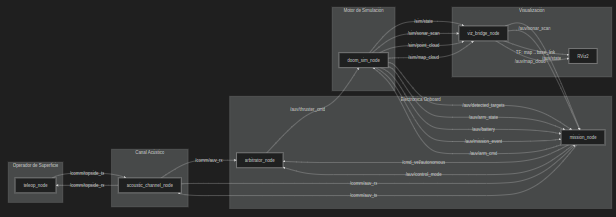
\includegraphics[width=\linewidth]{rqt_graph.png}
    \caption{Topología ROS\,2 del sistema (\texttt{rqt\_graph}). Los nodos se agrupan en cinco dominios funcionales: Topside, Canal Acústico, Onboard, Simulador y Visualización.}
    \label{fig:topologia}
\end{figure}

La Tabla~\ref{tab:nodos} resume los nodos y sus responsabilidades.

\begin{table}[H]
\centering
\caption{Nodos ROS\,2 del sistema y sus roles.}
\label{tab:nodos}
\scriptsize
\begin{tabular}{@{}lp{5.2cm}@{}}
\toprule
\textbf{Nodo} & \textbf{Responsabilidad} \\
\midrule
\texttt{doom\_sim\_node} & Motor de simulación: física, renderizado Pygame, publicación de sensores \\
\texttt{teleop\_node} & Interfaz de operador en terminal con dashboard \\
\texttt{acoustic\_channel\_node} & Canal bidireccional con latencia y pérdida de paquetes \\
\texttt{arbitrator\_node} & Multiplexor de comandos Manual/Auto \\
\texttt{mission\_node} & Lógica de autonomía onboard con máquina de estados \\
\texttt{viz\_bridge\_node} & Puente con delay para RViz\,2 (TF + PointCloud) \\
\bottomrule
\end{tabular}
\end{table}

La decisión de utilizar exclusivamente tópicos Pub/Sub ---sin Servicios ni Acciones ROS\,2--- responde a la naturaleza fundamentalmente asíncrona del dominio. Un Servicio ROS\,2 es bloqueante: el cliente espera la respuesta del servidor. En un escenario donde la comunicación puede tardar segundos o perderse, este patrón provocaría bloqueos inaceptables en el bucle de control. Las Acciones, aunque asíncronas con soporte de \textit{feedback}, introducirían complejidad de gestión de estados que se resuelve de forma más directa mediante la máquina de estados del nodo de misión combinada con eventos en tópicos.

\subsection{Motor de Simulación}

El nodo \texttt{doom\_sim\_node} ejecuta un bucle principal a 20\,Hz que integra tres subsistemas: la física subacuática, el motor de renderizado y la interfaz ROS\,2.

\subsubsection{Motor de Física}

La física modela un AUV con tres grados de libertad controlables: avance lineal, rotación en yaw y movimiento vertical. En lugar de asignar velocidad directamente desde los comandos recibidos, el sistema aplica un modelo de \textbf{inercia hidrodinámica acumulativa}. Los comandos del \texttt{/auv/thruster\_cmd} (tipo \texttt{Twist}) se interpretan como fuerzas que aceleran el vehículo:

\begin{lstlisting}[caption={Modelo de aceleraci\'on y drag hidr\'aulico.}, label={lst:physics}]
# Aceleracion: los comandos acumulan velocidad
self.linear_vel += cmd.linear.x * FORCE_LINEAR
self.angular_vel += cmd.angular.z * FORCE_ANGULAR
self.z_vel += cmd.linear.z * FORCE_Z

# Drag hidrodinamico: decaimiento por tick
self.linear_vel *= WATER_DRAG_LINEAR   # 0.92
self.angular_vel *= WATER_DRAG_ANGULAR # 0.85
self.z_vel *= WATER_DRAG_LINEAR
\end{lstlisting}

El factor de \textit{drag} $d = 0.92$ implica que, en ausencia de fuerzas externas, la velocidad decae exponencialmente como $v(t) = v_0 \cdot d^t$, produciendo un movimiento suave con inercia perceptible. La colisión se resuelve mediante comprobación directa contra el mapa de celdas y verificación de proximidad con obstáculos, incluyendo una lógica que permite al vehículo escapar si ya se encuentra dentro del radio de colisión.

El modelo de batería implementa un consumo heterogéneo: un drenaje base de $0.001$ unidades por tick más contribuciones proporcionales a la velocidad lineal ($|\dot{x}| \times 0.005$), angular ($|\dot{\theta}| \times 0.01$) y vertical ($|\dot{z}| \times 0.01$).

\subsubsection{Motor de Renderizado}

El renderizado emplea la técnica de \textit{raycasting}~\cite{lodev_raycasting}, donde 120 rayos se lanzan desde la posición del AUV en un arco de 60° (\texttt{FOV = $\pi/3$}). Para cada rayo, se avanza iterativamente en incrementos de 5 píxeles hasta detectar una pared o alcanzar la profundidad máxima (100 unidades). La distancia perpendicular se calcula aplicando corrección de \textit{fisheye}:

\begin{equation}
d_{\perp} = d_{\text{raw}} \cdot \cos(\theta_{\text{player}} - \theta_{\text{ray}})
\label{eq:fisheye}
\end{equation}

La altura de la columna renderizada es inversamente proporcional a la distancia: $h = 21000 / (d_{\perp} + \epsilon)$. Los obstáculos dinámicos (barcos, criaturas) y estáticos (arrecifes, minas) se renderizan como \textit{sprites} billboard con formas diferenciadas por tipo. Los \textit{targets} de recolección se dibujan como círculos con un indicador de orientación (línea roja).

Un efecto colateral del raycasting es la revelación progresiva del mapa (\textit{fog of war}): cada celda atravesada por un rayo se marca como explorada en una matriz booleana \texttt{fog\_map[100$\times$100]}, que controla la visibilidad tanto en el minimap de sonar como en los datos de exportación.

\begin{figure}[H]
    \centering
    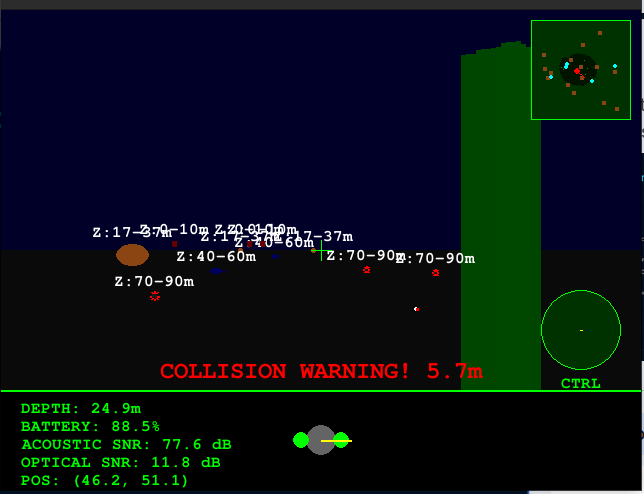
\includegraphics[width=\linewidth]{sim_screenshot.png}
    \caption{Interfaz del simulador DOOM AUV. La vista principal muestra el renderizado por \textit{raycasting} 2.5D. El HUD inferior muestra profundidad, batería y SNR. El minimap superior derecho presenta la cobertura del sonar con \textit{fog of war}. El brazo robótico con gripper aparece en la parte inferior central.}
    \label{fig:interface}
\end{figure}

\subsection{Canal de Comunicación Acústica}

El nodo \texttt{acoustic\_channel\_node} implementa un canal bidireccional entre el operador de superficie (\textit{topside}) y la electrónica onboard del AUV. Cada mensaje JSON que entra por \texttt{/comm/topside\_tx} (downlink) o \texttt{/comm/auv\_tx} (uplink) se encola con un retardo calculado como:

\begin{equation}
\tau = \frac{R}{c_s} + U(0.01, 0.05) \quad [\text{s}]
\label{eq:delay}
\end{equation}

donde $R$ es la distancia al AUV, $c_s = 1500$\,m/s la velocidad del sonido en agua y $U(a,b)$ una componente uniforme aleatoria que modela el \textit{jitter} del procesamiento. Adicionalmente, cada paquete tiene una probabilidad de pérdida del 5\%, independiente e idénticamente distribuida.

El módulo \texttt{CommunicationPhysics} implementa el modelo completo de SNR acústico según la Ecuación~\ref{eq:tl} con la absorción de Thorp (Ecuación~\ref{eq:thorp}) a $f = 25$\,kHz y $SL = 185$\,dB re 1\,$\mu$Pa. El SNR óptico se modela con una atenuación exponencial ($c = 0.08$\,m$^{-1}$, rango 100\,m) correspondiente a agua oceánica clara. Un modelo simplificado de escintilación introduce cortes aleatorios del 5\% que simulan el efecto de ondas internas.

\subsection{Arquitectura de Control}

\subsubsection{Arbitraje de Comandos}

El nodo \texttt{arbitrator\_node} opera como un multiplexor temporal: en cada tick de su bucle a 20\,Hz, publica en \texttt{/auv/thruster\_cmd} el último comando recibido de la fuente activa (manual o autónoma), siempre que dicho comando sea reciente ($< 0.5$\,s). Si no hay comandos recientes, publica un \texttt{Twist} nulo, lo que el drag hidráulico traduce en deceleración progresiva.

\subsubsection{Subsunción de Seguridad}

El nodo \texttt{mission\_node} implementa una jerarquía de prioridades inspirada en la arquitectura de subsunción~\cite{brooks1986}. Las capas de seguridad operan \textbf{en todos los modos}, incluyendo el manual, y pueden forzar el cambio a modo autónomo:

\begin{enumerate}[leftmargin=*,itemsep=2pt]
    \item \textbf{EMERGENCY\_REVERSE} ($d < 1.5$\,m): Retroceso puro durante 2\,s. Prioridad máxima.
    \item \textbf{AVOID\_CRITICAL} ($d < 3.0$\,m): Retroceso con rotación hacia el lado con mayor espacio libre, durante 3\,s.
    \item \textbf{BATTERY\_FAILSAFE} (batería $< 10\%$): Fuerza ascenso de emergencia.
    \item \textbf{Estados de misión} (EXPLORE, APPROACH, ALIGN, etc.): Solo activos en modo AUTO.
\end{enumerate}

La dirección de evasión se determina en tiempo real comparando la suma de rangos del sonar en los hemicampos izquierdo y derecho:

\begin{lstlisting}[caption={Determinaci\'on de la direcci\'on de evasi\'on.}, label={lst:evasion}]
mid = len(scan.ranges) // 2
left_sum  = sum(scan.ranges[mid:])
right_sum = sum(scan.ranges[:mid])
turn_dir = 1.0 if left_sum > right_sum else -1.0
\end{lstlisting}

\subsection{Misión Autónoma}

La autonomía onboard se estructura como una máquina de estados finita con seis estados principales (Figura~\ref{fig:fsm}).

\begin{figure}[H]
    \centering
    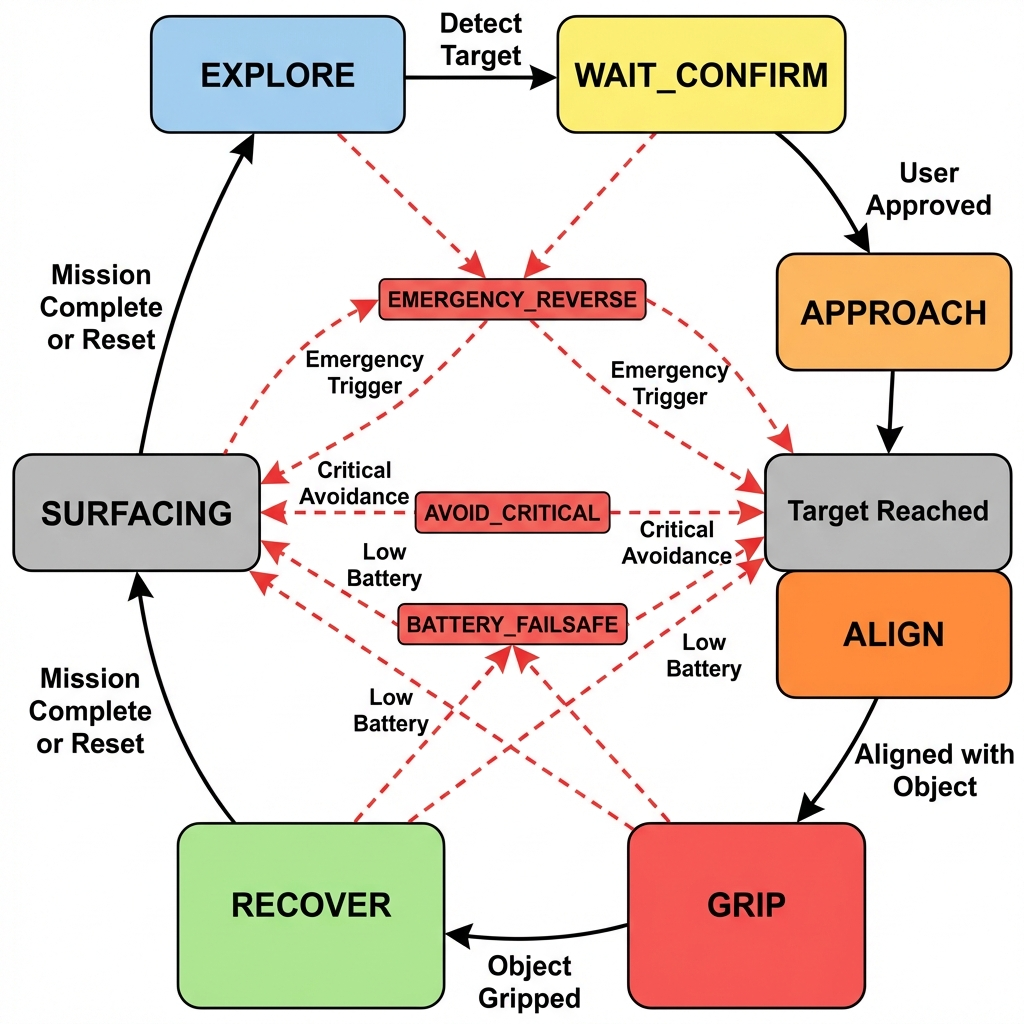
\includegraphics[width=\linewidth]{fsm_diagram.png}
    \caption{Máquina de estados de la misión autónoma. Las transiciones de seguridad (líneas rojas) pueden interrumpir cualquier estado.}
    \label{fig:fsm}
\end{figure}

\textbf{EXPLORE:} El AUV sigue un patrón \textit{lawnmower} (barrido sistemático en zigzag) definido por una lista de waypoints en una rejilla de paso 20 unidades. La navegación emplea un controlador proporcional en \textit{yaw} con ganancia $K_p = 0.5$, saturado en $\pm 1.0$\,rad/s. La velocidad lineal se reduce a $0.2$ cuando el error angular es grande ($|\psi_e| > 0.5$\,rad) para evitar avance durante giros pronunciados.

\textbf{WAIT\_CONFIRM:} Cuando el simulador publica un target visible en \texttt{/auv/detected\_targets}, el \textit{mission\_node} transiciona a espera de confirmación, publicando telemetría actualizada. El operador debe enviar una confirmación (\texttt{confirm}) o rechazo (\texttt{reject}) a través del canal acústico. Los targets rechazados se almacenan para evitar redetección.

\subsubsection{Control de Aproximación (APPROACH)}

El estado APPROACH implementa un \textbf{controlador proporcional dual} que gobierna simultáneamente la velocidad lineal y la velocidad angular del AUV, con el objetivo de converger al target minimizando la distancia euclídea $d = \sqrt{\Delta x^2 + \Delta y^2}$ y el error de heading $\psi_e$.

El error de heading se calcula como la diferencia normalizada al intervalo $(-\pi, \pi]$:

\begin{equation}
\psi_e = \left(\text{atan2}(\Delta y, \Delta x) - \psi_{\text{auv}} + \pi\right) \bmod 2\pi - \pi
\label{eq:heading_error}
\end{equation}

donde $\psi_{\text{auv}} = 2 \cdot \text{atan2}(q_z, q_w)$ se extrae del cuaternión de orientación. La ley de control angular aplica:

\begin{equation}
\omega = \text{clamp}\left(\psi_e \cdot K_\omega,\; -\omega_{\max},\; \omega_{\max}\right)
\label{eq:approach_angular}
\end{equation}

con $K_\omega = 0.3$ y $\omega_{\max} = 0.5$\,rad/s. Esta ganancia fue reducida respecto al valor original de $0.5$ para prevenir giros agresivos que causaban sobrepasamiento y oscilaciones alrededor del target.

La velocidad lineal implementa un \textbf{esquema de conmutación con zona muerta angular}:

\begin{equation}
v = \begin{cases}
0 & \text{si } |\psi_e| > 0.2 \text{ rad} \\
\text{clamp}\left(0.3 \cdot d,\; 0.1,\; 0.5\right) & \text{en caso contrario}
\end{cases}
\label{eq:approach_linear}
\end{equation}

La conmutación en $|\psi_e| = 0.2$\,rad es crítica: \textbf{el AUV no avanza si no está apuntando al target}. Esto previene la deriva lateral que, sin inercia nula, acumularía velocidad perpendicular al heading deseado. La velocidad proporcional a la distancia ($0.3 \cdot d$) proporciona deceleración natural en la fase final, evitando el rebasamiento.

La transición a ALIGN se activa cuando se cumplen tres condiciones conjuntas: $d < 1.5$\,m, $|\Delta z| < 2.0$\,m (profundidad) y $|\psi_e| < 0.3$\,rad. Un freno de emergencia ($v = 0$) se aplica incondicionalmente a $d < 0.5$\,m para prevenir colisión con el target.

\subsubsection{Alineamiento y Visual Servoing (ALIGN)}

El estado ALIGN constituye el módulo de control más complejo del sistema. A diferencia de APPROACH, que opera en el espacio cartesiano del mundo, ALIGN utiliza \textbf{visual servoing basado en imagen} (\textit{Image-Based Visual Servoing}, IBVS): el error se define directamente en coordenadas de pantalla $(u, v)$ del target renderizado, y la acción de control se aplica sobre los actuadores del brazo robótico.

\textbf{Congelación del cuerpo.} Al entrar en ALIGN, el AUV detiene completamente su movimiento de cuerpo ($v = 0$, $\omega = 0$). Esta decisión de diseño evita un \textit{loop} de realimentación indeseado: cualquier rotación del cuerpo desplaza la imagen del target en pantalla, lo que provocaría correcciones del brazo, que a su vez alterarían la posición relativa. Mantener el cuerpo estático desacopla los dos sistemas de control.

\textbf{Control del brazo.} El brazo se controla mediante comandos discretos (``left'', ``right'', ``up'', ``down'', ``rot\_left'', ``rot\_right'') publicados a 10\,Hz. Para determinar qué comando enviar, el algoritmo implementa una \textbf{política de prioridad con alternancia}:

\begin{lstlisting}[caption={Bucle de visual servoing del estado ALIGN.}, label={lst:align}]
# 1. Rotacion - Prioridad ALTA
if abs(diff_deg) >= 5.0:
    if abs(diff_deg) >= 15.0 or tick_even:
        cmd = "rot_right" if diff_deg > 0
              else "rot_left"
# 2. Posicion en X (pantalla)
elif abs(cur_x - target_x) > 5:  # px
    cmd = "right" if cur_x < target_x
          else "left"
# 3. Posicion en Y (pantalla)
elif abs(cur_y - target_y) > 5:  # px
    cmd = "down" if cur_y < target_y
          else "up"
else:
    pos_aligned = True
\end{lstlisting}

La rotación del gripper se computa como diferencia angular normalizada entre la orientación absoluta del target (extraída del cuaternión) y el ángulo actual del gripper:

\begin{equation}
\Delta\theta = \left(\theta_{\text{target}} - \theta_{\text{gripper}} + 180°\right) \bmod 360° - 180°
\label{eq:gripper_rotation}
\end{equation}

La política de alternancia (\texttt{tick\_even}) permite que, cuando la rotación está ``suficientemente cerca'' ($|\Delta\theta| < 15°$) pero no ``perfecta'' ($|\Delta\theta| \geq 5°$), el sistema alterne entre correcciones de rotación y posición en \textit{ticks} pares e impares. Esto evita que el brazo quede bloqueado en un ciclo de correcciones puramente rotacionales.

\textbf{Avance lento (\textit{creep forward}).} Solo cuando la posición y rotación del brazo están alineadas pero la distancia 3D al target es $> 1.2$\,m, el sistema aplica un avance lineal mínimo de $v = 0.1$, acercando el cuerpo al objeto sin perder la alineación. Esta lógica actúa como un controlador \textit{bang-bang} de proximidad.

La Tabla~\ref{tab:control_params} sintetiza los parámetros de control de ambos estados.

\begin{table}[H]
\centering
\caption{Parámetros de los controladores de APPROACH y ALIGN.}
\label{tab:control_params}
\scriptsize
\begin{tabular}{@{}llcc@{}}
\toprule
\textbf{Estado} & \textbf{Parámetro} & \textbf{Valor} & \textbf{Unidad} \\
\midrule
APPROACH & $K_\omega$ (heading) & 0.3 & -- \\
APPROACH & $\omega_{\max}$ & 0.5 & rad/s \\
APPROACH & Rango $v$ & [0.1, 0.5] & m/s \\
APPROACH & Zona muerta angular & 0.2 & rad \\
APPROACH & Dist.\ transición & 1.5 & m \\
\midrule
ALIGN & Tol.\ rotación (estricta) & 5.0 & $°$ \\
ALIGN & Tol.\ rotación (alternancia) & 15.0 & $°$ \\
ALIGN & Tol.\ posición pantalla & 5 & px \\
ALIGN & $v$ creep & 0.1 & m/s \\
ALIGN & Dist.\ grip ($d_{3D}$) & 1.2 & m \\
\bottomrule
\end{tabular}
\end{table}

\subsubsection{Verificación y Cierre del Gripper (GRIP)}

La transición de ALIGN a GRIP se activa cuando las tres condiciones son simultáneamente verdaderas: $|\Delta\theta| < 5°$, posición centrada en pantalla ($|u_e| < 5$\,px y $|v_e| < 5$\,px), y $d_{3D} < 1.2$\,m. Tras la transición, el módulo de renderizado verifica de forma independiente tres condiciones: distancia 3D $< 1.5$\,m, error angular del gripper $< 30°$, y distancia en pantalla $< 50$\,px. Si la captura falla, el sistema regresa a ALIGN paso 0 y reabre el gripper para reintentar.

\subsection{Entorno Procedural}

El \texttt{MapManager} genera un mundo submarino procedural sobre un mapa de $100 \times 100$ celdas. La Tabla~\ref{tab:obstacles} detalla la distribución de obstáculos.

\begin{table}[H]
\centering
\caption{Distribución de obstáculos y targets.}
\label{tab:obstacles}
\scriptsize
\begin{tabular}{@{}lcccl@{}}
\toprule
\textbf{Tipo} & \textbf{N} & \textbf{Prof. (m)} & \textbf{Dinámica} & \textbf{ID Color} \\
\midrule
Barcos & 10 & 0--10 & Sí & Rojo (3) \\
Criaturas & 10 & 40--60 & Sí & Azul (4) \\
Arrecifes & 15 & 17--37 & No & Marrón (5) \\
Minas & 15 & 70--90 & No & Gris (6) \\
Targets & 5 & 5--95 & No & Cyan \\
\bottomrule
\end{tabular}
\end{table}

% ============================================================================
\section{Proceso de Desarrollo Iterativo}
\label{sec:desarrollo}

El sistema fue desarrollado mediante un proceso iterativo de refinamiento continuo que abarcó más de quince ciclos de desarrollo. A continuación se documentan los principales hitos y bloqueos técnicos resueltos, organizados cronológicamente.

\subsection{Fase 1: Arquitectura Base}

La primera iteración estableció los componentes fundamentales: el nodo de simulación con renderizado por \textit{raycasting}, el \textit{teleop\_node} con comunicación directa mediante tópicos \texttt{Twist}, y un mapa estático con paredes fijas. En esta fase, el control manual publicaba directamente en el tópico \texttt{/cmd\_vel}, sin canal acústico intermedio. La física asignaba la velocidad de forma instantánea, sin inercia.

\subsection{Fase 2: Comunicación Acústica y Dashboard}

Se introdujo el \texttt{acoustic\_channel\_node} como intermediario obligatorio para toda la comunicación operador-AUV. El \textit{teleop\_node} fue rediseñado para empaquetar comandos como JSON y transmitirlos por \texttt{/comm/topside\_tx}. El dashboard de terminal se implementó con códigos ANSI para mostrar telemetría en tiempo real.

Un bloqueo importante fue la detección de la \textbf{desconexión del enlace acústico}: el dashboard mostraba ``DISCONNECTED'' intermitentemente porque la verificación de tiempo de último paquete no se actualizaba correctamente. La solución consistió en actualizar \texttt{last\_packet\_time} ante \textit{cualquier} JSON válido recibido, independientemente de su contenido.

\subsection{Fase 3: Autonomía y Evasión de Obstáculos}

La implementación del \texttt{mission\_node} con la máquina de estados y la arquitectura de subsunción requirió múltiples iteraciones. El primer problema crítico fue que el \textbf{autopiloto no tomaba el control} cuando era necesario: las capas de seguridad no forzaban el modo AUTO en situaciones de emergencia. La solución fue añadir la publicación explícita en \texttt{/auv/control\_mode} desde las capas de seguridad.

\subsection{Fase 4: Control del Brazo y Estabilización}

La fase de alineamiento del brazo robótico para la captura de targets fue la más problemática y requirió al menos seis ciclos de refinamiento:

\begin{itemize}[leftmargin=*,itemsep=2pt]
    \item \textbf{Gripper desalineado:} El gripper se posicionaba consistentemente a la izquierda del target. Se refinó la lógica de \textit{visual servoing} para equilibrar rotación y ajuste posicional.
    \item \textbf{Distancia de captura:} Inicialmente fijada en 3\,m, resultaba excesiva. Se redujo iterativamente a 1.5\,m (verificación en \texttt{renderer.py}) y 1.2\,m (transición en \texttt{mission\_node}).
    \item \textbf{Oscilación vertical:} El controlador de profundidad con ganancia $K_p = 1.0$ causaba oscilaciones verticales que impedían la captura. Se redujo a $K_p = 0.3$ para un control más suave.
    \item \textbf{Velocidad del brazo:} La velocidad de rotación y desplazamiento del brazo se ajustó para permitir un control preciso sin sobrepasamiento.
    \item \textbf{Gripper que no cerraba:} Se relajó la tolerancia angular de $5°$ a $30°$ para permitir la captura con alineamientos aproximados, más realistas operativamente.
\end{itemize}

\subsection{Fase 5: Realismo Acústico y Exportación 3D}

En la fase final, se eliminaron los canales de comunicación directa residuales, asegurando que el 100\% del control manual pasara por el canal acústico con latencia y pérdida de paquetes. Se implementó la exportación del mapa explorado en formato OBJ (Wavefront) como mesh 3D, complementando los formatos PCD y PNG ya existentes.

% ============================================================================
\section{Pruebas y Resultados}
\label{sec:resultados}

\subsection{Protocolo de Pruebas}

Las pruebas se ejecutaron en un entorno Ubuntu 22.04 LTS con ROS\,2 Humble Hawksbill, Python 3.10 y Pygame 2.x. El sistema se inicia mediante el archivo launch:

\begin{lstlisting}[language=bash, caption={Secuencia de ejecuci\'on.}]
$ colcon build
$ source install/setup.bash
$ ros2 launch doom_auv_sim doom_sim.launch.py
# En terminal separado:
$ ros2 run doom_auv_sim teleop_node
\end{lstlisting}

\subsection{Resultados Funcionales}

La Tabla~\ref{tab:resultados} resume los resultados obtenidos en las pruebas del sistema completo.

\begin{table}[H]
\centering
\caption{Resultados de las pruebas funcionales.}
\label{tab:resultados}
\scriptsize
\begin{tabular}{@{}lcc@{}}
\toprule
\textbf{Métrica} & \textbf{Valor} & \textbf{Estado} \\
\midrule
Targets recolectados (auto) & 5/5 & \checkmark \\
Evasión de obstáculos & Funcional & \checkmark \\
Battery failsafe & Activa $< 10\%$ & \checkmark \\
Comunicación acústica & Delay + 5\% loss & \checkmark \\
Fog of war & Progresivo & \checkmark \\
Exportación PCD/PNG/OBJ & Post-misión & \checkmark \\
Frecuencia de simulación & 20\,Hz estable & \checkmark \\
Frecuencia de control & 10\,Hz estable & \checkmark \\
\bottomrule
\end{tabular}
\end{table}

\subsection{Análisis del Control de Profundidad}

La reducción de la ganancia del controlador de profundidad de $K_p = 1.0$ a $K_p = 0.3$ eliminó las oscilaciones verticales observadas en versiones anteriores. El error de profundidad en estado estacionario se mantiene por debajo de $\pm 0.5$\,m, lo cual es suficiente para la transición de APPROACH a ALIGN (tolerancia de 2.0\,m).

\subsection{Análisis del Canal Acústico}

El delay medio observado se sitúa entre 70 y 300\,ms dependiendo de la distancia al punto de partida. La pérdida de paquetes del 5\% introduce saltos perceptibles en el dashboard de telemetría sin comprometer la estabilidad del sistema, gracias al diseño asíncrono de la arquitectura.

\begin{figure}[H]
    \centering
    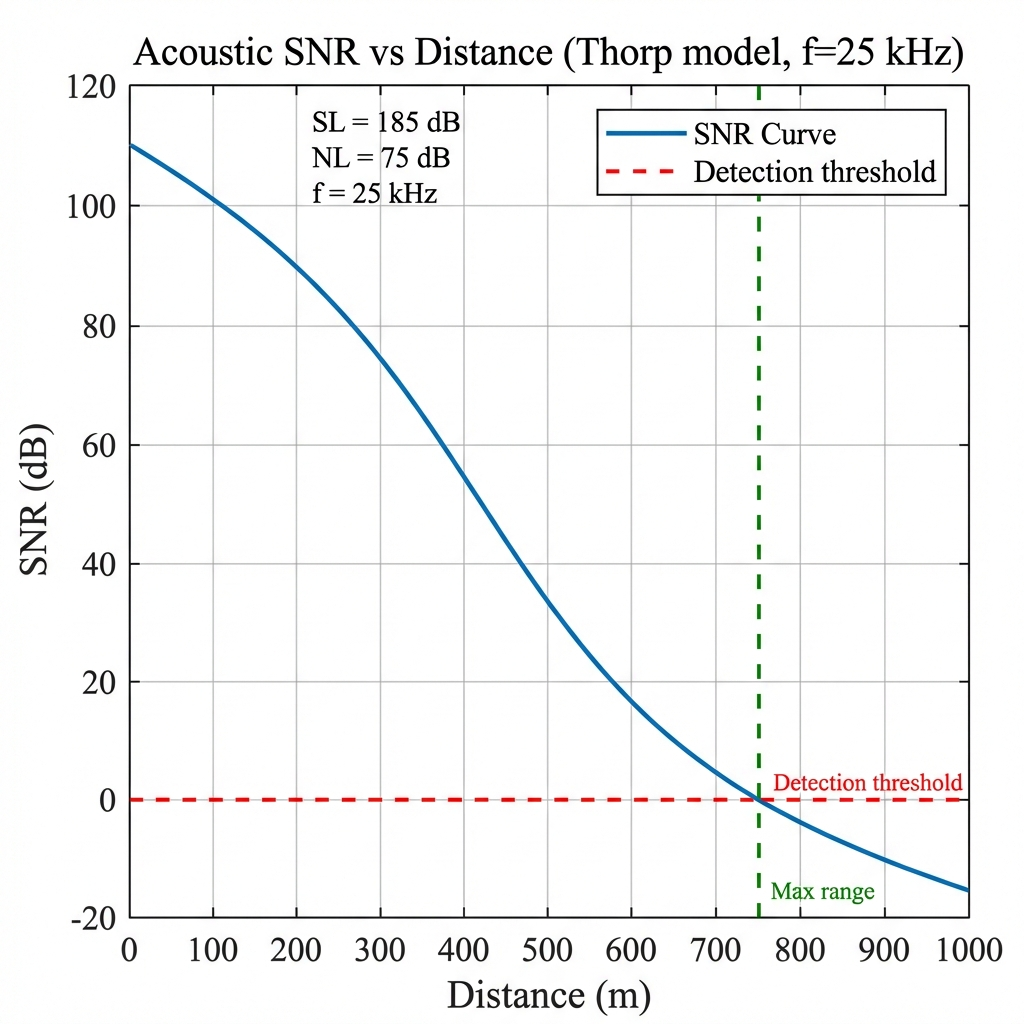
\includegraphics[width=\linewidth]{snr_graph.png}
    \caption{SNR acústico calculado en función de la distancia usando la fórmula de absorción de Thorp a 25\,kHz.}
    \label{fig:snr}
\end{figure}

% ============================================================================
\section{Conclusiones y Trabajo Futuro}
\label{sec:conclusiones}

El presente trabajo ha demostrado la viabilidad de un simulador de AUV ligero construido sobre ROS\,2 que reproduce las restricciones operativas esenciales del dominio submarino. El sistema integra con éxito un motor de renderizado por \textit{raycasting}, un canal de comunicación acústica con modelo de propagación basado en Thorp, una arquitectura de control con jerarquía de subsunción para seguridad, y un módulo de autonomía onboard capaz de completar misiones de exploración y recolección.

El proceso de desarrollo iterativo puso de manifiesto la importancia del \textit{tuning} de parámetros en robótica: la estabilidad del control de profundidad, la tolerancia de captura del gripper y la velocidad del brazo robótico requirieron múltiples ciclos de ajuste empírico. La documentación de estos ciclos constituye un aporte pedagógico valioso, ya que ilustra la realidad del desarrollo en robótica más allá de la arquitectura teórica.

\subsection{Limitaciones Identificadas}

\begin{itemize}[leftmargin=*,itemsep=2pt]
    \item \textbf{Navegación reactiva:} La ausencia de un planificador global (e.g., Nav2 con A*) limita la capacidad del AUV para rodear obstáculos complejos. La navegación en línea recta con evasión temporal puede resultar en trayectorias subóptimas o bloqueos en configuraciones geométricas adversas.
    \item \textbf{Pérdida de paquetes i.i.d.:} El modelo de pérdidas independientes no captura la correlación temporal observada en canales acústicos reales. Un modelo de Markov (Gilbert-Elliott) proporcionaría mayor realismo.
    \item \textbf{Planificación 2D:} Tanto Nav2 como la mayoría de planificadores ROS\,2 están diseñados para navegación 2D, lo cual limita su aplicabilidad directa a un AUV que opera en tres dimensiones.
\end{itemize}

\subsection{Trabajo Futuro}

\begin{itemize}[leftmargin=*,itemsep=2pt]
    \item Integración de Nav2 para planificación de trayectorias 2D horizontales, manteniendo el controlador de profundidad actual.
    \item Modelo de canal acústico correlacionado (Gilbert-Elliott) y aplicación activa del shift Doppler a los datos de control.
    \item Extensión a escenarios multi-AUV cooperativos con protocolos TDMA de acceso al canal acústico.
    \item Adición de modelos de corrientes marinas que afecten a la navegación y a la propagación acústica.
    \item Integración con \texttt{slam\_toolbox} para cartografía simultánea a partir del sonar simulado.
\end{itemize}

% ============================================================================
% REFERENCIAS
% ============================================================================
\begin{thebibliography}{10}

\bibitem{stojanovic2009}
M. Stojanovic y J. Preisig,
``Underwater Acoustic Communication Channels: Propagation Models and Statistical Characterization,''
\textit{IEEE Commun. Mag.}, vol.~47, no.~1, pp.~84--89, 2009.

\bibitem{uuvsim2016}
M. M. M. Manhaes, S. A. Scherer, M. Voss, L. R. Douat y T. Rauschenbach,
``UUV Simulator: A Gazebo-based package for underwater intervention and multi-robot simulation,''
\textit{Proc. IEEE OCEANS}, 2016.

\bibitem{stonefish2020}
M. Cieślak,
``Stonefish: An Advanced Open-Source Simulation Tool Designed for Marine Robotics, with a ROS Interface,''
\textit{Proc. IEEE OCEANS}, 2019.

\bibitem{thorp1967}
W. H. Thorp,
``Analytic Description of the Low-Frequency Attenuation Coefficient,''
\textit{J. Acoust. Soc. Am.}, vol.~42, no.~1, p.~270, 1967.

\bibitem{urick1983}
R. J. Urick,
\textit{Principles of Underwater Sound}, 3\textsuperscript{a} ed.
Peninsula Publishing, 1983.

\bibitem{brooks1986}
R. A. Brooks,
``A Robust Layered Control System for a Mobile Robot,''
\textit{IEEE J. Robot. Autom.}, vol.~2, no.~1, pp.~14--23, 1986.

\bibitem{lodev_raycasting}
Lode Vandevenne,
``Raycasting Tutorial,''
\url{https://lodev.org/cgtutor/raycasting.html}, accedido Feb.~2026.

\bibitem{ros2docs}
Open Robotics,
``ROS 2 Documentation: Humble Hawksbill,''
\url{https://docs.ros.org/en/humble/}, 2022.

\bibitem{quigley2009}
M. Quigley \textit{et al.},
``ROS: an open-source Robot Operating System,''
\textit{Proc. ICRA Workshop on Open Source Software}, 2009.

\bibitem{nav2}
S. Macenski \textit{et al.},
``The Marathon 2: A Navigation System,''
\textit{Proc. IEEE/RSJ IROS}, 2020.

\end{thebibliography}

\end{document}
